\section{Design pattern}

\subsection{Model View Presenter}
\begin{itemize}
\item \textbf{Scopo e descrizione:}
Il \textit{pattern\ped{G}} architetturale \textit{Model View Presenter} (MVP) è un derivato del \textit{Model View Controller} (MVC), focalizzato sulla valorizzazione della logica della presentazione. Entrambi i pattern hanno lo sopo di disaccoppiare la logica dell'applicazione dalla rappresentazione grafica.\\
Il \textit{pattern\ped{G}} MVP prevede la suddivisione dell'applicazione in tre componenti:
\begin{itemize}
\item \textbf{Model:} Definisce il modello dati e le regole di accesso e di modifica;
\item \textbf{View:} Si occupa della rappresentazione dell'interfaccia utente;
\item \textbf{Presenter:} Contiene la logica dell'applicazione, si occupa delle comunicazioni tra vista e modello e dell'aggiornamento della vista.
\end{itemize}
\begin{figure}[H] \centering 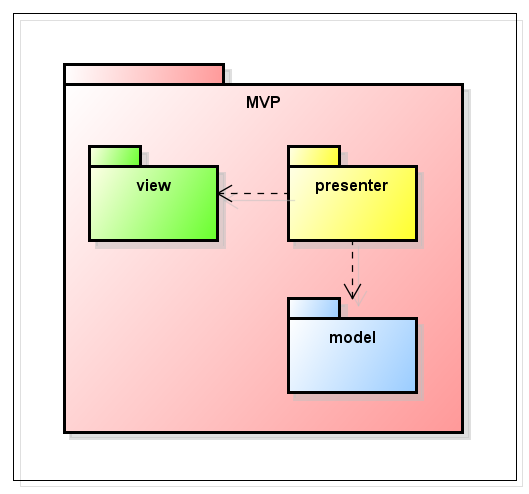
\includegraphics[scale=1]{./pattern/mvp.png} \caption{Diagramma UML pattern MVP}
\end{figure}
\item \textbf{Contesto d'uso:}
Il \textit{pattern\ped{G}} \textit{Model View Presenter} (MVP) è la architettura di base del progetto.
\end{itemize}

\subsection{Facade}
\begin{itemize}
\item \textbf{Scopo e descrizione:}
Il \textit{pattern\ped{G}} strutturale \textit{Facade} prevede l'utilizzo di un'interfaccia unica e semplice per un sottosistema complesso, diminuendo la complessità del sistema;
\begin{figure}[H] \centering 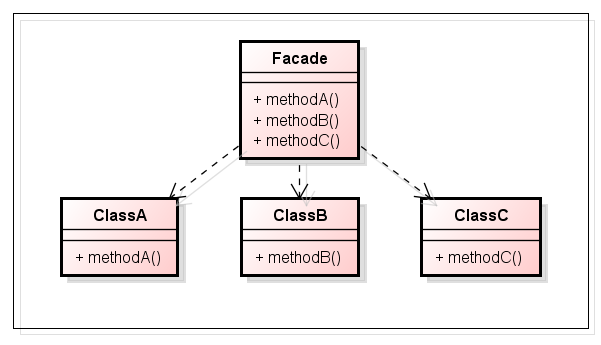
\includegraphics[scale=1]{./pattern/facade.png} \caption{Diagramma UML pattern Facade}
\end{figure}
\item \textbf{Contesto d'uso:}
Il \textit{pattern\ped{G}} \textit{Facade} è stato utilizzato nei \textit{package\ped{G} sequenziatore::server::presenter}, \textit{sequenziatore::server::model}, \textit{sequenziatore::client::presenter::user::logic} e \textit{sequenziatore::client::view::user}.
\end{itemize}

\subsection{Data Access Object}
\begin{itemize}
\item \textbf{Scopo e descrizione:}
Il \textit{pattern\ped{G}} \textit{Data Access Object} (DAO) permette alla \textit{business logic\ped{G}} di essere indipendente dall'implementazione della persistenza dei dati.
Il \textit{pattern\ped{G}} DAO è caratterizzato dai seguenti componenti:
\begin{itemize}
\item \textbf{Data Access Object:}
Realizza l'acesso fisico alla sorgente dei dati in modo trasparente al resto dell'applicazione;
\item \textbf{Object Transfer:}
Rappresenta l'oggeto utilizzato per il trasferimento dei dati, sia in lettura, sia in scrittura.
\end{itemize}
\begin{figure}[H] \centering 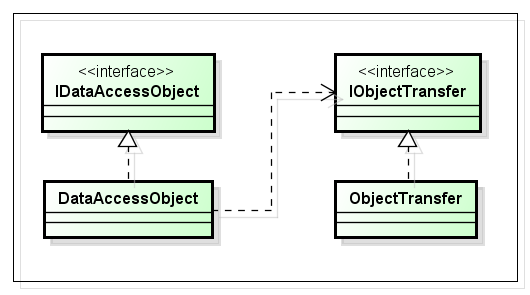
\includegraphics[scale=1]{./pattern/dao.png} \caption{Diagramma UML pattern DAO}
\end{figure}
\item \textbf{Contesto d'uso:}
Il \textit{pattern\ped{G}} DAO è stato utilizzato nei \textit{package\ped{G} sequenziatore::server::model::daouser}, \textit{sequenziatore::server::model::daoprocessowner}, \textit{sequenziatore::server::model::daoprocess} e \textit{sequenziatore::server::model::daostep}. 
\end{itemize}